\documentclass[a4paper]{article}
\usepackage[utf8]{inputenc}
\usepackage{amsmath}
\usepackage{amsfonts}
\usepackage{graphicx}
\usepackage{amssymb}
\setlength{\parindent}{0in}
\usepackage{fancyhdr}

\begin{document}

\pagestyle{fancy}
\rhead{David Nápravník - přezdívka ":)"}

\setcounter{section}{2}
\section{du}
\subsection{sachovnice}
z sachovnice si udelejme jednu dlouhou cestu ktera prochazi kazdym polickem:\\
\begin{tabular}{|l|l|l|l|l|l|} 
\hline
\multicolumn{1}{|l}{\#} & \multicolumn{1}{l}{}   & \multicolumn{1}{l}{\#} & \multicolumn{1}{l}{}   & \multicolumn{1}{l}{\#} &     \\ 
\cline{2-5}
                        & \multicolumn{1}{l}{\#} &                        & \multicolumn{1}{l}{\#} &                        & \#  \\
R                       &                        & \#                     &                        & \#                     &     \\
                        & \#                     &                        & \#                     &                        & \#  \\
\#                      &                        & \#                     &                        & \#                     & R   \\
                        & \#                     &                        & \#                     &                        & \#  \\
\multicolumn{1}{|l}{\#} &                        & \multicolumn{1}{l}{\#} &                        & \multicolumn{1}{l}{\#} &     \\
\hline
\end{tabular}\\
kde \# je cerne policko, cesta je ohranicena a R jsou vymazana policka\\
\\
pak mame ruzne barvy policek na obou koncich cesty a tudiz lze poskladat domino.

\subsection{tok cesta a rez}
\textbf{tvrzeni plati}\\
reseni vychazi z definice minimalniho rezu, nebot velikost minimalniho rezu odpovida velikosti toku

\subsection{kruznice}
pokud mame kazdy vrchol stupne 2 a pridame dalsi 2 hrany (na kazdou stranu jednu), tak graf bude 4-souvisly jak hranove tak i vrcholove.

\subsection{souvisly graf}
Ja bych radeji dokazal opak a to sice ze existuje graf, ktery ma mene nez 30 hran, je souvisly, 
rovinny a presto muze jeho vrchol mit stupen vetsi nez 4.\\
Vytvorme kruznici o vice nez 4 vrcholech a pak jeden bod uprostred, pote napojime kazdy vrchol z kruznice na bod uprostred a dostaneme rovinny, souvisly graf s mene nez 30 hranami  jez ma vrchol stupne vice nez 4.

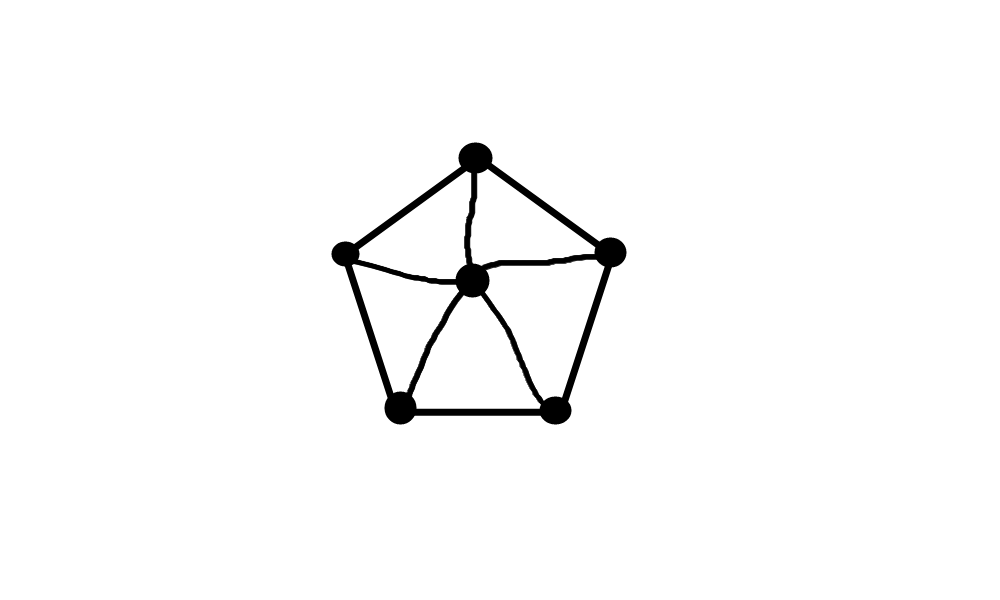
\includegraphics[height=3cm]{circle}

\subsection{magicka krychle}
\textbf{ano, plati}\\
Definujme si jednotkovou krychly jakozto krychly, ktera ma na pricne diagonale jednicky.\\
pak muzeme provadet upravy podobne na maticich, neboli prohozeni poradi dvou ctvercu(jedne vrstvy) a dostaneme stale krychli sily 1\\
Pak dve krychle sily 1 ktere vzniknou rozlozenim krychle sily dva bodou pouze nejakou permutaci jednotkove krychle.

\end{document}